Hier folgen Sequenzdiagramme, die den Ablauf des Programms und deren Methoden visualisieren.
Die genauen Szenarios sind dem Pflichtenheft zu entnehmen.
\section{Überprüfen des Logs von Algorithmen}
\graphicspath{{./img/sequ/}}
\textbf{Vorbedingung:} Bilder eines Modells wurden erstellt. \newline
\textbf{Ergebnis:} Der Nutzer kann anhand der Meldungen im Log die Eignung der gewählten Algorithmen für die Bilder einschätzen und Verbesserungen an den Algorithmen vornehmen. \newline
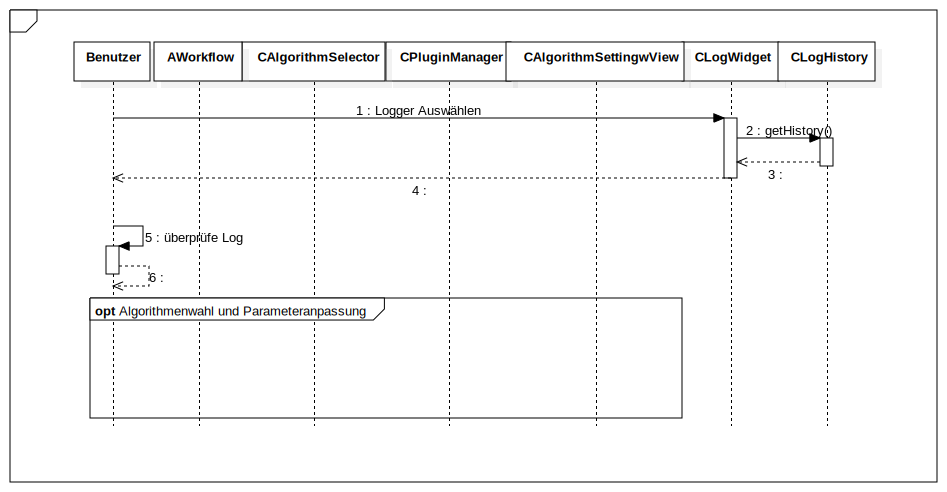
\includegraphics[width=\linewidth]{Anwendungsfall_Logger}
\newpage
\section{Erzeugung eines 3D Modells}
\textbf{Vorbedingung:} Bilder des Modells wurden erstellt. \newline
\textbf{Ergebnis:} Fertiges 3D-Modell liegt zur weiteren Verarbeitung in anderer Software vor. \newline
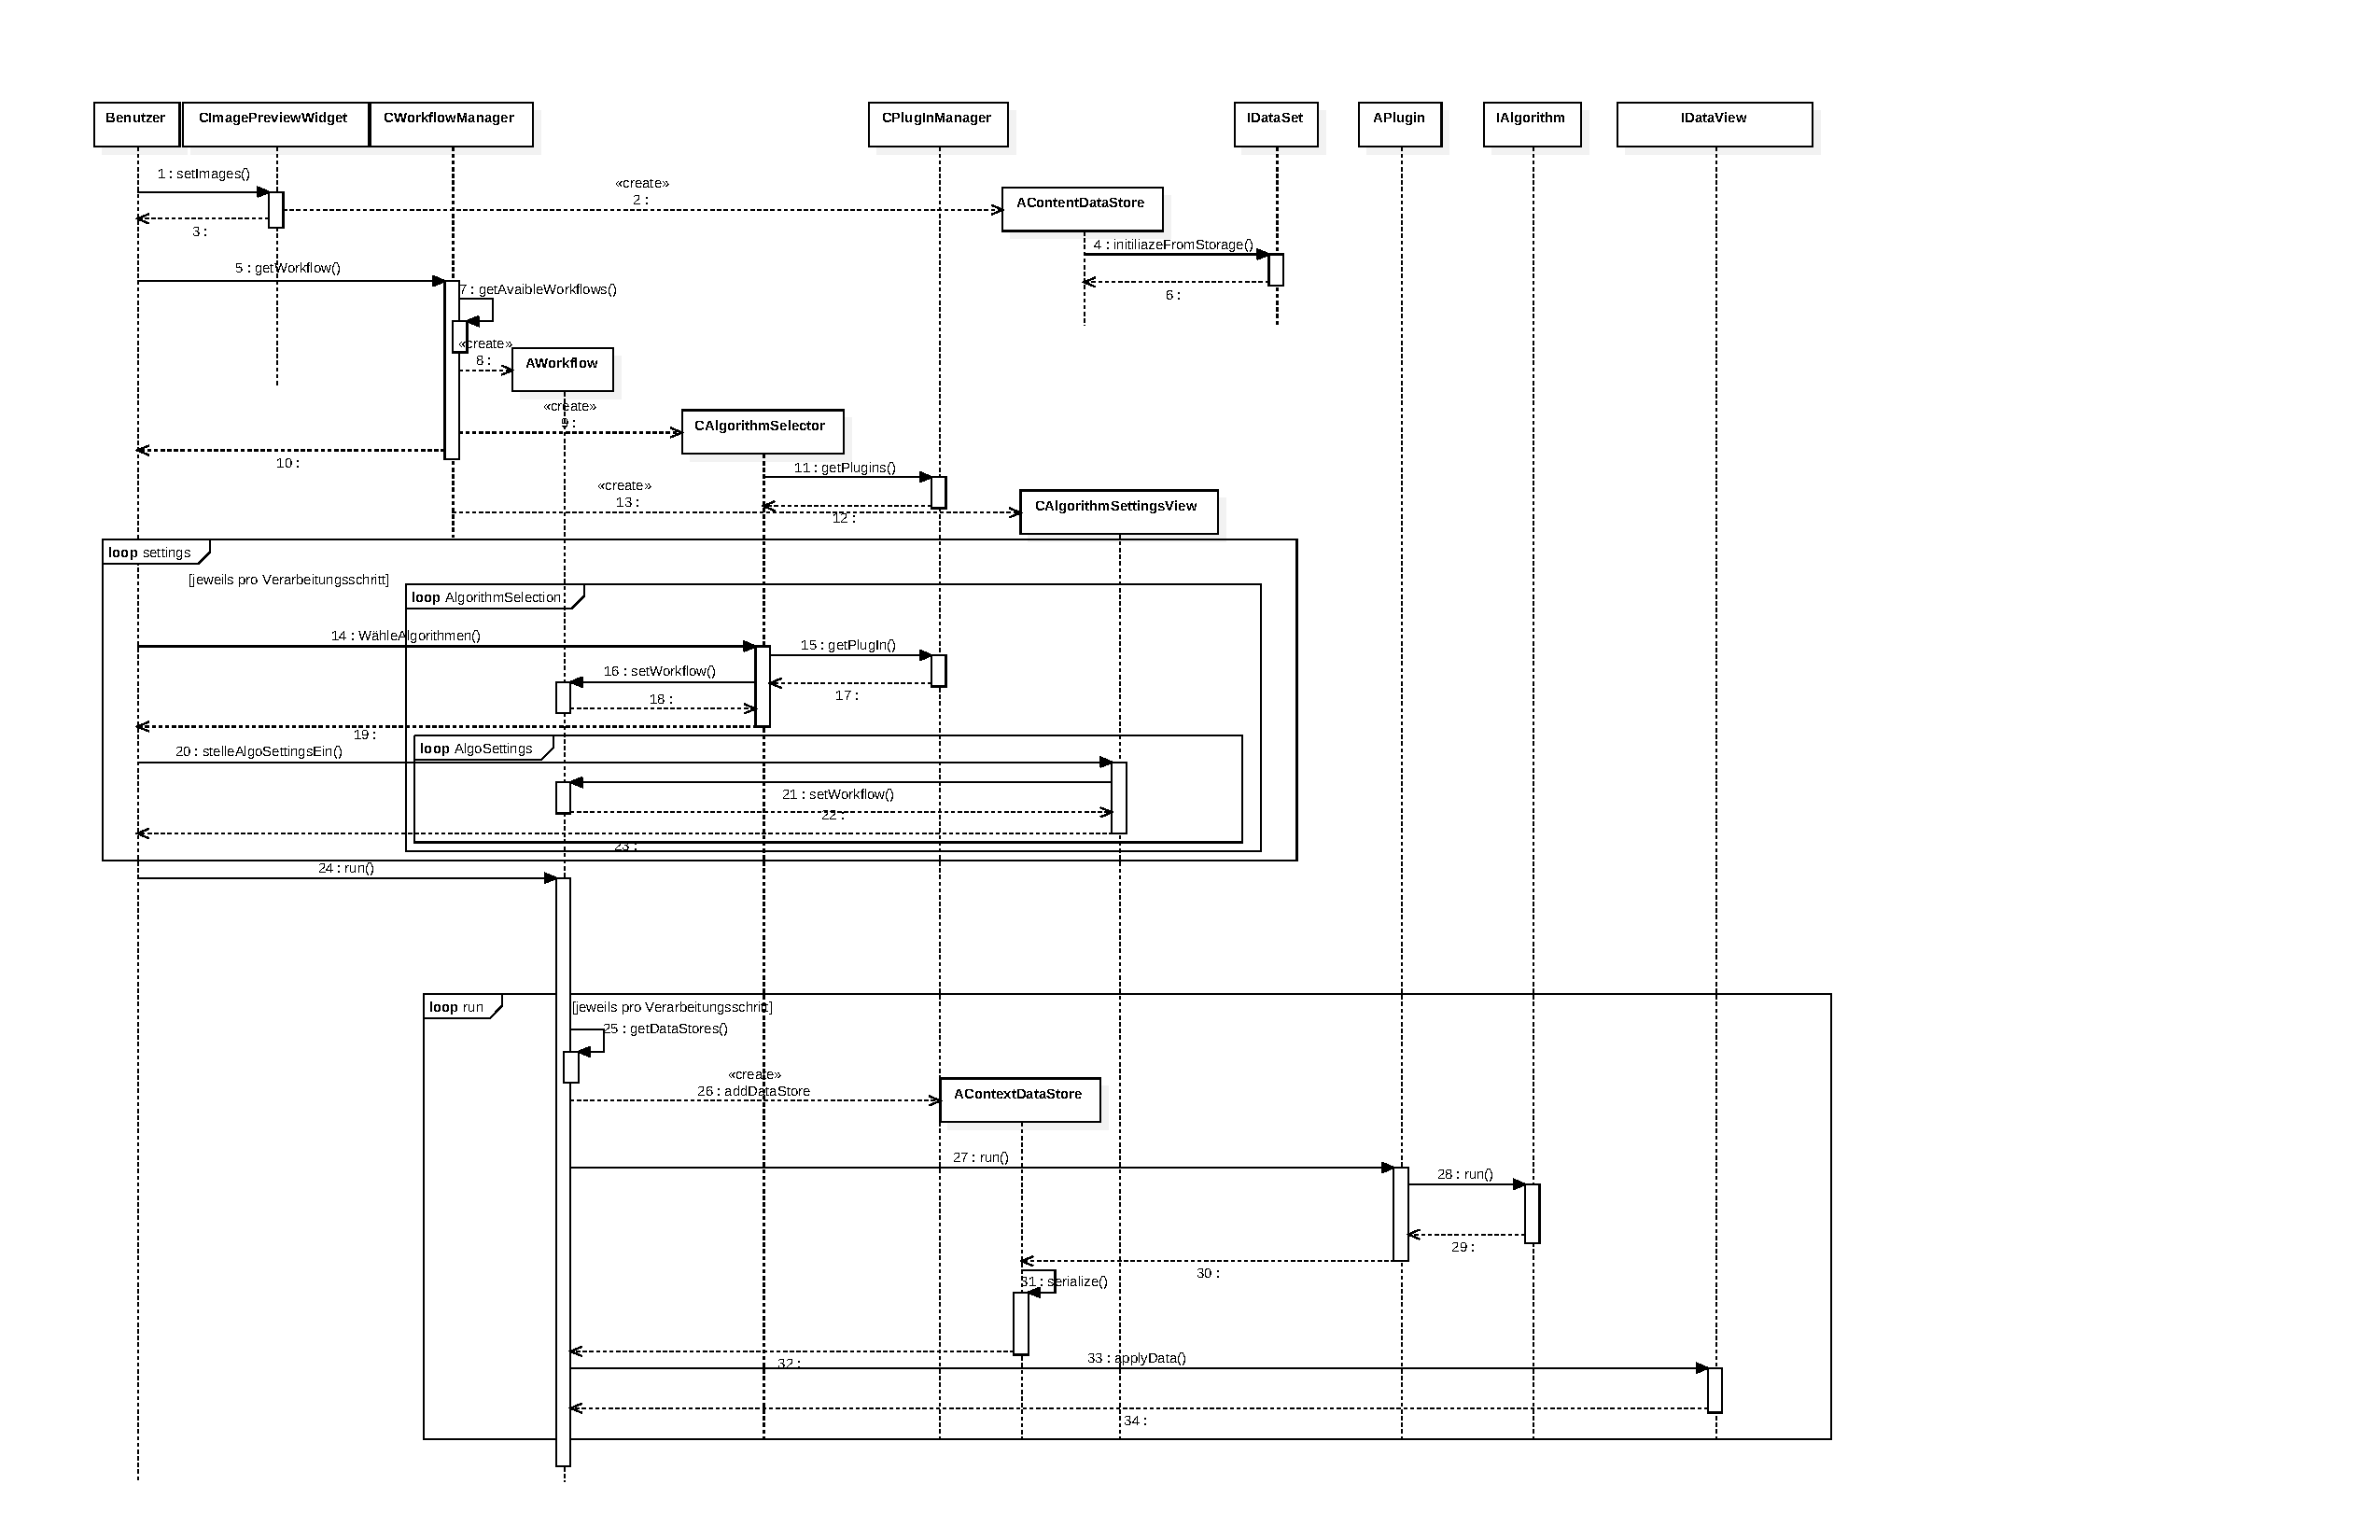
\includegraphics[width=\linewidth]{ErzeugenEines3DModels}